\newcommand{\fileInfectorTagResultsAucTable}{
    \begin{table}[H]
        \centering
        \begin{tabular}{|p{2,8cm}||P{2,2cm} P{2,2cm} P{2,2cm} P{2,2cm}|}
            \hline
            File-infector Tag & ALOHA\newline (M/B only) & ALOHA & Joint\newline Embedding & Proposed\newline Model \\
            \hline
            AUC-ROC & - & 0.982$\pm$0.002 & 0.983$\pm$0.001 & \textBF{0.986$\pm$0.001} \\
            \hline
        \end{tabular}
        \caption{AUC-ROC (Area Under Curve) of the different models for the \textbf{File-infector Tag} prediction task. Results were aggregated over \textBF{3} training runs with different weight initializations and minibatch orderings. Best results are shown in \textbf{bold}.} \label{tab:fileInfectorTag_auc}
    \end{table}
}

\newcommand{\fileInfectorTagResultsAtFprTable}{
    \begin{center}
        \begin{longtable}[c]{|P{3,2cm}||P{1,8cm} P{1,8cm} P{1,8cm} P{1,8cm} P{1,8cm}|}
            \hline
            File-infector Tag & \multicolumn{5}{c|}{{FPR}} \\
            & $10^{-5}$ & $10^{-4}$ & $10^{-3}$ & $10^{-2}$ & $10^{-1}$ \\
            \hline
            \endfirsthead

            \caption*{\raggedright ...continued from previous page} \\
            \hline
            File-infector Tag & \multicolumn{5}{c|}{\textbf{FPR}} \\
            & $10^{-5}$ & $10^{-4}$ & $10^{-3}$ & $10^{-2}$ & $10^{-1}$ \\
            \hline
            \endhead

            \caption*{\raggedleft ...continued on next page} \\
            \endfoot

            \caption{Mean and standard deviation results (TPR, Accuracy, Recall, Precision and F1-Score) of the different models for the \textbf{File-infector Tag} prediction task at different \textbf{FPR}s (\textit{False Positive Rates}). Results were aggregated over \textBF{3} training runs with different weight initializations and minibatch orderings. Best results are shown in \textbf{bold}. Under \textbf{TPR} results are also presented the percentage reduction in mean detection error and in ROC curve standard deviation introduced by the \textit{Proposed Model} with respect to both \textit{ALOHA} model and \textit{Joint Embedding}.} \label{tab:fileInfectorTag_results_at_fpr} \\
            \endlastfoot

            \multicolumn{6}{|c|}{\textbf{TPR}} \\
            \hline
            ALOHA (M/B only) & - & - & - & - & - \\
            ALOHA & \textBF{0.375$\pm$0.199} & 0.481$\pm$0.173 & 0.799$\pm$0.018 & 0.851$\pm$0.008 & 0.946$\pm$0.013 \\
            Joint Embedding & 0.294$\pm$0.166 & \textBF{0.541$\pm$0.131} & 0.797$\pm$0.025 & 0.857$\pm$0.009 & 0.952$\pm$0.013 \\
            Proposed Model & 0.360$\pm$0.155 & 0.532$\pm$0.060 & \textBF{0.829$\pm$0.022} & \textBF{0.872$\pm$0.011} & \textBF{0.956$\pm$0.013} \\
            \hline
            Error Reduction wrt\newline ALOHA (M/B only) & - & - & - & - & - \\
            Error Reduction wrt\newline ALOHA & -2.4\% & 9.8\% & 14.9\% & 14.1\% & 18.5\% \\
            Error Reduction wrt\newline Joint Embedding & 9.3\% & -2.0\% & 15.8\% & 10.5\% & 8.3\% \\
            \hline
            Std Reduction wrt\newline ALOHA (M/B only) & - & - & - & - & - \\
            Std Reduction wrt\newline ALOHA & 22.1\% & 65.3\% & -22.2\% & -37.5\% & 0.0\% \\
            Std Reduction wrt\newline Joint Embedding & 6.6\% & 54.2\% & 12.0\% & -22.2\% & 0.0\% \\
            \hline
            \multicolumn{6}{|c|}{\textbf{Accuracy}} \\
            \hline
            ALOHA (M/B only) & - & - & - & - & - \\
            ALOHA & \textBF{0.899$\pm$0.032} & 0.916$\pm$0.028 & 0.967$\pm$0.003 & 0.968$\pm$0.001 & 0.907$\pm$0.002 \\
            Joint Embedding & 0.886$\pm$0.027 & \textBF{0.926$\pm$0.021} & 0.966$\pm$0.004 & 0.969$\pm$0.001 & 0.908$\pm$0.002 \\
            Proposed Model & 0.897$\pm$0.025 & 0.924$\pm$0.010 & \textBF{0.972$\pm$0.004} & \textBF{0.971$\pm$0.002} & \textBF{0.909$\pm$0.002} \\
            \hline
            \multicolumn{6}{|c|}{\textbf{Recall}} \\
            \hline
            ALOHA (M/B only) & - & - & - & - & - \\
            ALOHA & \textBF{0.374$\pm$0.199} & 0.481$\pm$0.173 & 0.799$\pm$0.018 & 0.851$\pm$0.008 & 0.946$\pm$0.013 \\
            Joint Embedding & 0.294$\pm$0.166 & \textBF{0.541$\pm$0.131} & 0.797$\pm$0.025 & 0.857$\pm$0.009 & 0.952$\pm$0.013 \\
            Proposed Model & 0.360$\pm$0.155 & 0.531$\pm$0.060 & \textBF{0.829$\pm$0.022} & \textBF{0.872$\pm$0.011} & \textBF{0.956$\pm$0.013} \\
            \hline
            \multicolumn{6}{|c|}{\textbf{Precision}} \\
            \hline
            ALOHA (M/B only) & - & - & - & - & - \\
            ALOHA & \textBF{1.000$\pm$0.000} & \textBF{0.999$\pm$0.000} & \textBF{0.994$\pm$0.000} & 0.943$\pm$0.000 & 0.646$\pm$0.003 \\
            Joint Embedding & \textBF{1.000$\pm$0.000} & \textBF{0.999$\pm$0.000} & \textBF{0.994$\pm$0.000} & 0.943$\pm$0.001 & 0.647$\pm$0.003 \\
            Proposed Model & \textBF{1.000$\pm$0.000} & \textBF{0.999$\pm$0.000} & \textBF{0.994$\pm$0.000} & \textBF{0.944$\pm$0.001} & \textBF{0.648$\pm$0.003} \\
            \hline
            \multicolumn{6}{|c|}{\textbf{F1 Score}} \\
            \hline
            ALOHA (M/B only) & - & - & - & - & - \\
            ALOHA & \textBF{0.517$\pm$0.195} & 0.632$\pm$0.150 & 0.886$\pm$0.011 & 0.894$\pm$0.004 & 0.767$\pm$0.006 \\
            Joint Embedding & 0.427$\pm$0.216 & 0.692$\pm$0.117 & 0.884$\pm$0.015 & 0.898$\pm$0.005 & 0.771$\pm$0.007 \\
            Proposed Model & 0.509$\pm$0.180 & \textBF{0.692$\pm$0.053} & \textBF{0.904$\pm$0.013} & \textBF{0.907$\pm$0.006} & \textBF{0.772$\pm$0.006} \\
            \hline
        \end{longtable}
    \end{center}
}

\newcommand{\fileInfectorTagResultsSummaryTable}{
    \begin{table}[H]
        \centering
        \begin{tabular}{|P{3,2cm}||P{1,8cm} P{1,8cm} P{1,8cm} P{1,8cm} P{1,8cm}|}
            \hline
            \multicolumn{6}{|c|}{File-infector Tag (at FPR $=1\%$)} \\
            \hline
            Model & TPR & Accuracy & Precision & Recall & F1 score \\
            \hline
            ALOHA (M/B only) & - & - & - & - & - \\
            ALOHA & 0.851$\pm$0.008 & 0.968$\pm$0.001 & 0.943$\pm$0.000 & 0.851$\pm$0.008 & 0.894$\pm$0.004 \\
            Joint Embedding & 0.857$\pm$0.009 & 0.969$\pm$0.001 & 0.943$\pm$0.001 & 0.857$\pm$0.009 & 0.898$\pm$0.005 \\
            Proposed Model & \textBF{0.872$\pm$0.011} & \textBF{0.971$\pm$0.002} & \textBF{0.944$\pm$0.001} & \textBF{0.872$\pm$0.011} & \textBF{0.907$\pm$0.006} \\
            \hline
        \end{tabular}
        \caption{Summary of the mean and standard deviation results of the different models for the \textbf{File-infector Tag} prediction task at \textbf{FPR} $=1\%$. Results were aggregated over \textBF{3} training runs with different weight initializations and minibatch orderings. Best results are shown in \textbf{bold}.} \label{tab:fileInfectorTag_result_summary}
    \end{table}
}

\newcommand{\fileInfectorTagRocAlohaMB}{
    \begin{figure}[H]
        \vspace*{-0.5cm}
        \centering
        \includegraphics[width=0.6\textwidth]{./results/file_infector_tag_roc_alohaMB.png}
        \vspace*{-0.2cm}
        \caption{ROC curve and AUC statistics of \textBF{ALOHA (M/B only)} model for the \textbf{File-infector Tag}. The line represents the \textit{mean} TPR at a given FPR, while the shaded region represents the \textit{standard deviation}. Statistics were computed over \textBF{3} training runs, each with random parameter initialization.}
        \label{fig:fileInfectorTagRocAlohaMB}
    \end{figure}
}

\newcommand{\fileInfectorTagRocAloha}{
    \begin{figure}[H]
        \vspace*{-0.5cm}
        \centering
        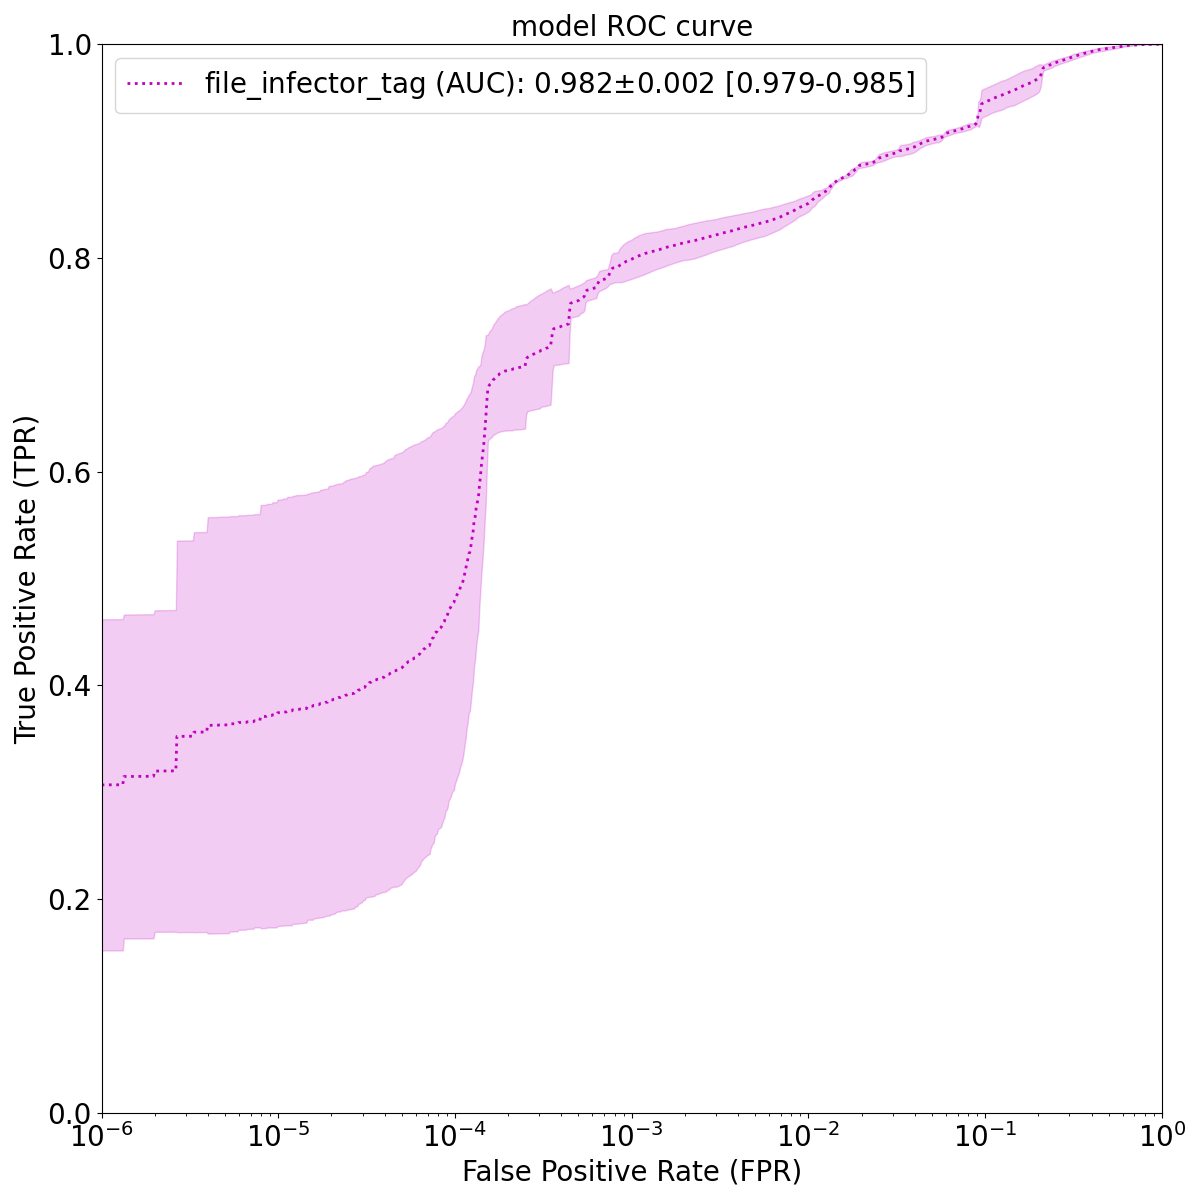
\includegraphics[width=0.6\textwidth]{./results/file_infector_tag_roc_aloha.png}
        \vspace*{-0.2cm}
        \caption{ROC curve and AUC statistics of \textBF{ALOHA} model for the \textbf{File-infector Tag}. The line represents the \textit{mean} TPR at a given FPR, while the shaded region represents the \textit{standard deviation}. Statistics were computed over \textBF{3} training runs, each with random parameter initialization.}
        \label{fig:fileInfectorTagRocAloha}
    \end{figure}
}

\newcommand{\fileInfectorTagRocJointEmbedding}{
    \begin{figure}[H]
        \vspace*{-0.5cm}
        \centering
        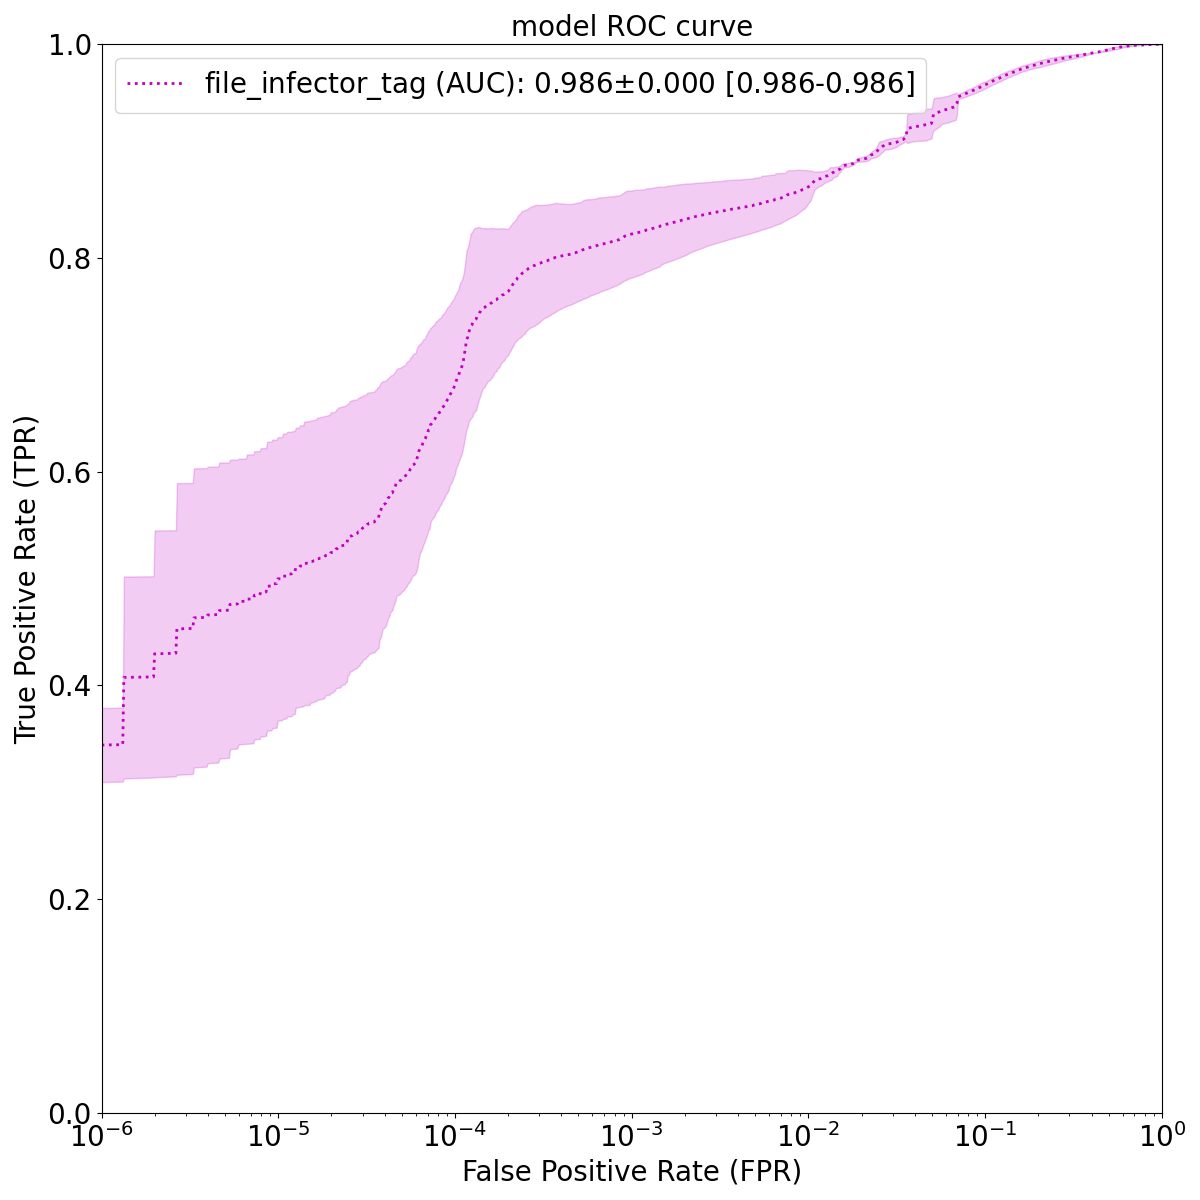
\includegraphics[width=0.6\textwidth]{./results/file_infector_tag_roc_jointEmbedding.png}
        \vspace*{-0.2cm}
        \caption{ROC curve and AUC statistics of \textBF{Joint Embedding} model for the \textbf{File-infector Tag}. The line represents the \textit{mean} TPR at a given FPR, while the shaded region represents the \textit{standard deviation}. Statistics were computed over \textBF{3} training runs, each with random parameter initialization.}
        \label{fig:fileInfectorTagRocJointEmbedding}
    \end{figure}
}

\newcommand{\fileInfectorTagRocProposedMethod}{
    \begin{figure}[H]
        \vspace*{-0.5cm}
        \centering
        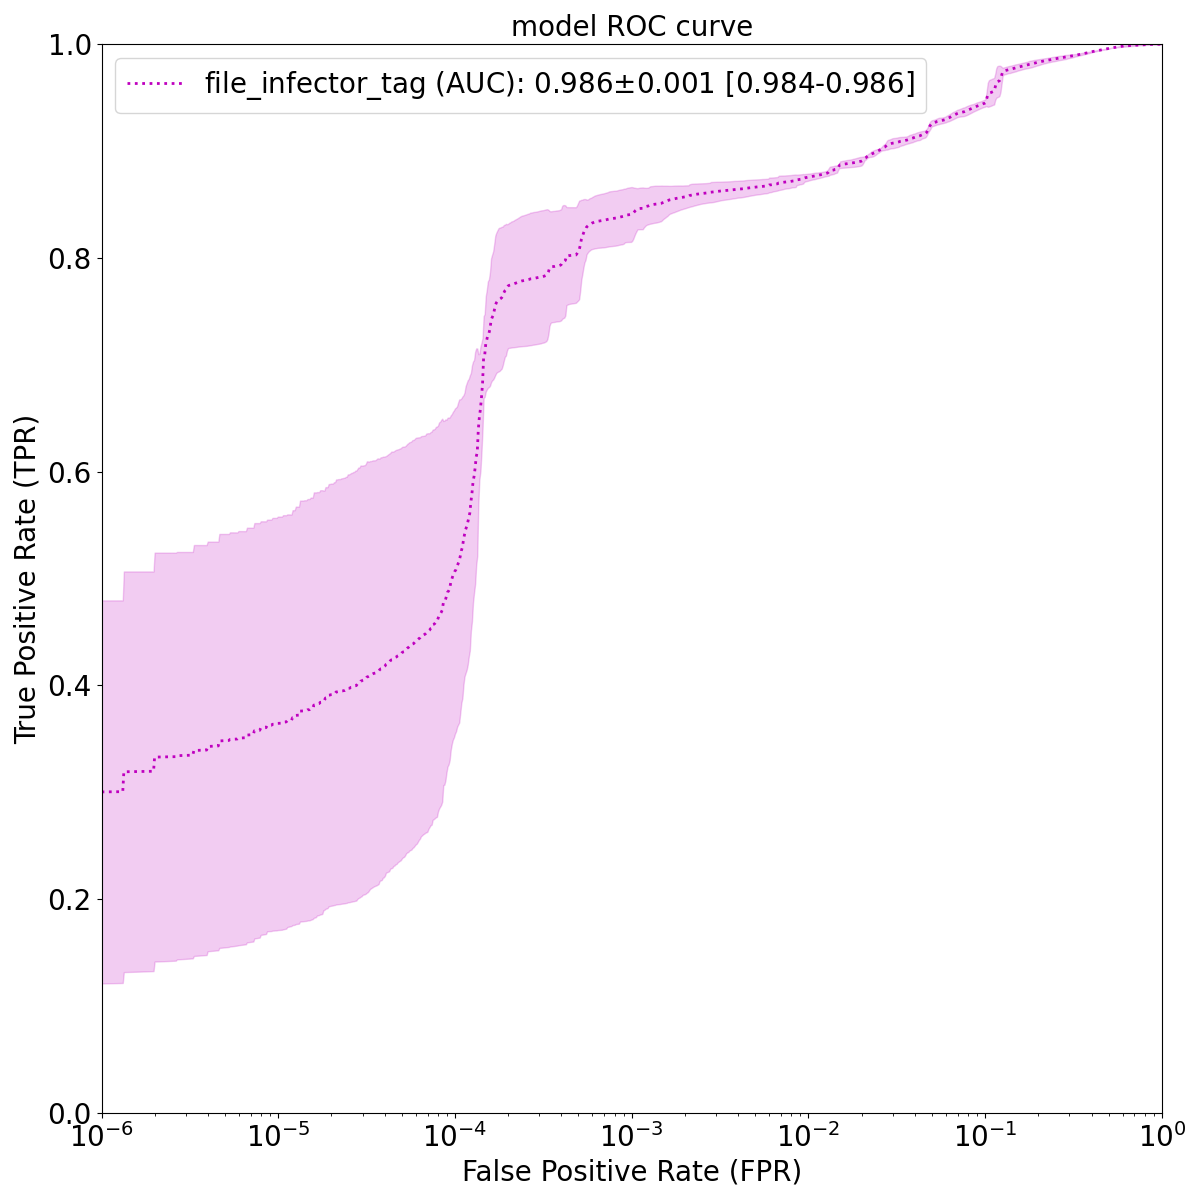
\includegraphics[width=0.6\textwidth]{./results/file_infector_tag_roc_proposedModel.png}
        \vspace*{-0.2cm}
        \caption{ROC curve and AUC statistics of \textBF{Proposed Model} for the \textbf{File-infector Tag}. The line represents the \textit{mean} TPR at a given FPR, while the shaded region represents the \textit{standard deviation}. Statistics were computed over \textBF{3} training runs, each with random parameter initialization.}
        \label{fig:fileInfectorTagRocProposedModel}
    \end{figure}
}
